\documentclass{article} \usepackage{chtt-notes} \usepackage{stmaryrd}
\usepackage{amssymb}

\usetikzlibrary{arrows}

\scribes{Travis Hance and Paul G\"olz} \week{9}
% The following command will let you cross-reference labels in the
% files week1.tex, week2.tex, \ldots, week\@week.tex, where if l is a
% label in ``weekN.tex'', then you can access the label using
% \cref{WN:l}.
\doXRs

% General remark: Using \cref{label} will fill in the appropriate
% environment name. For example, ``\begin{lemma}\label{lem:foo}
%   ...\end{lemma} By \cref{lem:foo}'' will produce ``Lemma 15 ... By
% lemma~15''

\newcommand{\lift}[1]{{#1}^{\Downarrow}}
\newcommand{\meet}[1]{\bigwedge\!#1}
\newcommand{\join}[1]{\bigvee\!#1}
\newcommand{\entails}{\vdash}
\newcommand{\G}{\Gamma}
\newcommand{\atype}[1]{#1~\mathit{type}}
\newcommand{\Nat}{\mathit{Nat}}
\newcommand{\circled}[1]{\text{\textcircled{#1}}}

\begin{document}
\maketitle
\section{Recap}

Last week, we formulated a mathematical account of the semantics of computational
type theory.

%\bibliographystyle{plainnat} \bibliography{ctt}

\section{Universes}%
\marginpar{March 22, 2018}%
To prove that zero and one are not equal, we need to be able to define a type family $P$ by induction on a natural number, which is not possible in ITT.

We might attempt to change this by adding natural recursion on the type level as a type constructor $\mathit{NATREC}$:
\[ \inferrule{\G \entails \atype{A_0} \quad \G, a: \Nat, b: \circled{?} \entails \atype{A_1} \quad \G \entails M : \Nat}{\G \entails \atype{\mathit{NATREC}(A_0; a,b.\; A_1)(M)}} \]
Even apart from the cumbersome repetition between definitions on the term and type level, it is not clear what ``type'' to give to $b$ in the premise.

What we need is a type of types, a \emph{universe} $\mathcal{U}$.
Membership in this type implies being a type:
\[ \inferrule{\G \entails A : \mathcal{U}}{\G \entails \atype{A}} \]
Then, we can do away with the distinction between terms and types, and use the usual rule for $\mathit{natrec}$ to type $P \coloneqq \mathit{natrec}(\top; \_, \_. \; \bot)$:
\[ \inferrule{\G \entails A_0 : \mathcal{U} \quad \G, a : \Nat, b : \mathcal{U} \entails A_1 : \mathcal{U} \quad \G \entails M : \Nat}{\G \entails \mathit{natrec}(A_0; a, b.\; A_1)(M)} : \mathcal{U} \]

To show, for example, that $P(\mathit{zero}) \equiv \top$, we lift the structural equality $P(\mathit{zero}) \equiv \top : \mathcal{U}$ using the following rule:
\[ \inferrule{\G \entails A \equiv B : \mathcal{U}}{\G \entails A \equiv B} \]

We then fill the universe with the types of ITT:
\[ \inferrule{}{\G \entails \Nat, \mathit{Bool}, \mathit{Void}, \mathit{Unit} : \mathcal{U}} \quad \quad \quad \inferrule{\G \entails A : \mathcal{U} \quad \G, a: A \entails B : \mathcal{U}}{\G \entails \Pi a : A.\; B, \Sigma a : A.\; B : \mathcal{U}}\]
\[ \inferrule{\G \entails A : \mathcal{U} \quad \G \entails M, N : A}{\G \entails \mathit{Id}_A(M, N) : \mathcal{U}} \]
And so forth.

Ideally, we would like $\mathcal{U}$ to encode all types.
However, we cannot set $\mathcal{U} : \mathcal{U}$ because this would be inconsistent by Russel's paradox.
To solve this problem, we define not just a single universe $\mathcal{U}$, but an infinite hierarchy of universes $\mathcal{U}_0: \mathcal{U}_1: \mathcal{U}_2 \dots$.
Every universe is maximal in the sense that it is closed under our type constructors by the afore-mentioned rules.
This hierarchy is cumulative as per the following rule:
\[ \inferrule{\G \entails M : \mathcal{U}_i}{\G \entails M : \mathcal{U}_{i + 1}}\]

It is worth pointing out that by now, types can include arbitrarily complicated computation.

\section{Higher identification}
If $\mathit{Id}_A$ should be a notion of equality, we would expect for example $\mathit{Id}_{\Nat \to \Nat}(f, g)$ to be inhabited iff $\Pi a: \Nat.\; \mathit{Id}_{\Nat}(f~a, g~a)$ is.

Now that we introduced universes, what should $\mathit{Id}_{\mathcal{U}}$ look like?
It would be natural to consider two types $A, B : \mathcal{U}$ as equal iff they are isomorphic, i.e., if there are functions $f : A \to B$ and $g : B \to A$ such that $g \circ f \circled{=} \mathit{id}$ and $f \circ g \circled{=} \mathit{id}$.
But which relation should we use for ``$\circled{=}$''?
Requiring structural equality as $g(f(a)) \equiv a$ is way to fine.
A slightly better step would be to require $\mathit{Id}_A(g(f(a)), a)$, and Vladimir Voevodsky's univalence goes into that direction. \medskip

In \cref{W7:sec:identitytypes} of Week~7, we considered different ways of constructing elements of identity types:
\begin{itemize}
    \item $\mathit{refl}_A(M) : \mathit{Id}_A (M, M)$. Leaving the type implicit, we suggestively set $\mathit{id} \coloneqq \mathit{refl}_A(M)$.
        We illustrate this as follows:
        \begin{center}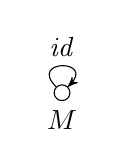
\begin{tikzpicture}[->,>=stealth',auto,node distance=2cm,every loop/.style={min distance=5mm,in=45,out=135,looseness=5}]
\node [circle, draw=black, inner sep=0pt, minimum size=2mm] (a) [label=below:$M$] {};
        \path[->] (a) edge  [loop above] node {$\mathit{id}$} ();\end{tikzpicture}\end{center}
    \item $\mathit{sym}_A(P) : \mathit{Id}_A (N, M)$ for $P : \mathit{Id}_A(M, N)$. Set $P^{-1} \coloneqq \mathit{sym}_A(P)$.
        \begin{center}\begin{tikzpicture}[->,>=stealth',auto,node distance=2cm,every loop/.style={min distance=5mm,in=45,out=135,looseness=5}]
\node [circle, draw=black, inner sep=0pt, minimum size=2mm] (a) [label=below:$M$] {};
\node [circle, draw=black, inner sep=0pt, minimum size=2mm] (b) [right=of a,label=below:$N$] {};
\draw [->, bend left] (a) to node [above] {$P$} (b);
        \draw [->, bend left] (b) to node [below] {$P^{-1}$} (a);\end{tikzpicture}\end{center}
    \item $\mathit{trans}_A(Q, R) : \mathit{Id}_A(M, P)$ for $Q : \mathit{Id}_A(M, N)$ and $R : \mathit{Id}_A(N, P)$. Denote this by $Q \circ R$.
        \begin{center}\begin{tikzpicture}[->,>=stealth',auto,node distance=2cm,every loop/.style={min distance=5mm,in=45,out=135,looseness=5}]
\node [circle, draw=black, inner sep=0pt, minimum size=2mm] (a) [label=below:$M$] {};
\node [circle, draw=black, inner sep=0pt, minimum size=2mm] (b) [right=of a,label=below:$N$] {};
\node [circle, draw=black, inner sep=0pt, minimum size=2mm] (c) [right=of b,label=below:$P$] {};
\draw [->] (a) to node [above] {$Q$} (b);
\draw [->] (b) to node [above] {$R$} (c);
        \draw [->, bend right] (a) to node [below] {$Q \circ R$} (c);\end{tikzpicture}\end{center}
\end{itemize}

We would expect this structure to respect the groupoid laws:
\begin{enumerate}
    \item \label{idrev} $\mathit{id}^{-1} \circled{=} \mathit{id}$
    \item \label{trid} $Q \circ \mathit{id} \circled{=} Q$
    \item \label{idtr} $\mathit{id} \circ R \circled{=} R$
    \item $P^{-1} \circ P \circled{=} \mathit{id}$
    \item \label{pinvid} $P \circ P^{-1} \circled{=} \mathit{id}$
    \item \label{assoc} $P \circ (Q \circ R) \circled{=} (P \circ Q) \circ R$
    \item $(P^{-1})^{-1} \circled{=} P$
\end{enumerate}
As we discussed in Week~7, choosing ``$\equiv$'' for ``$\circled{=}$'' only satisfies some of these laws.
For example, property~\ref{idrev} is true, whereas at most one out of properties~\ref{trid} and \ref{idtr} holds–––depending on the exact program used to implement transitivity.

To get the groupoid structure, we instead choose $\mathit{Id}_{\mathit{Id}_A}$ for ``$\circled{=}$'':

For instance, consider Law~\ref{pinvid}:
Suppose that we have $P : \mathit{Id}_A(M, N)$ and thus $P^{-1} : \mathit{Id}_A(n, M)$.
Then, by using $\mathit{id}^{-1} \equiv \mathit{id}$ and $\mathit{id} \circ \mathit{id} \equiv \mathit{id}$, one verifies that
\[J_{a,\_,p.\; \mathit{Id}_{\mathit{Id}_A(a,a)}(p \circ p^{-1}, \mathit{refl}_A(a))}(a.\; \mathit{refl}_{\mathit{Id}_A(a,a)}(\mathit{refl}_A(a)))(P) : \mathit{Id}_{\mathit{Id}_A(M, M)}(P \circ P^{-1}, \mathit{refl}_A(M)).\]

Or consider Law~\ref{assoc}:
\begin{center}\begin{tikzpicture}[->,>=stealth',auto,node distance=2cm,every loop/.style={min distance=5mm,in=45,out=135,looseness=5}]
\node [circle, draw=black, inner sep=0pt, minimum size=2mm] (a) [label=below:$S$] {};
\node [circle, draw=black, inner sep=0pt, minimum size=2mm] (b) [right=of a] {};
\node [circle, draw=black, inner sep=0pt, minimum size=2mm] (c) [right=of b] {};
\node [circle, draw=black, inner sep=0pt, minimum size=2mm] (d) [right=of c,label=below:$F$] {};
\draw [->] (a) to node [above] {$P$} (b);
\draw [->] (b) to node [above] {$Q$} (c);
\draw [->] (c) to node [above] {$R$} (d);
\draw [->, bend left] (a) to node [above] {$P \circ Q$} (c);
\draw [->, bend right] (b) to node [below] {$Q \circ R$} (d);
\draw [->, out=50, in=130] (a) to node [above] {$(P \circ Q) \circ R$} (d);
\draw [->, out=-50, in=-130] (a) to node [below] {$P \circ (Q \circ R)$} (d);\end{tikzpicture}\end{center}
Again, given $P, Q, R$, we can find a term of type $\mathit{Id}_{\mathit{Id}_A(S, F)}((P \circ Q) \circ R, P \circ (Q \circ R))$.
Borrowing intuitions from homotopy theory, this term can be thought of as a continuous deformation (a \emph{homotopy}) of the path corresponding to $(P \circ Q) \circ R$ into the path corresponding to $P \circ (Q \circ R)$.

Generally, the groupoid laws hold ``up to higher identification''.
We call the nesting depth of $\mathit{Id}_{\mathit{Id}_{._{._{.}}}}$ its dimension.
Again, in the language of homotopy, this corresponds to going from points (dimension 0) to paths between points (dimension 1) to paths between paths between points (dimension 2) and so forth.
Since the groupoid laws for objects of some dimension hold up to an equivalence of one higher dimension, the iterated $\mathit{Id}$s form a so-called \emph{$\infty$-groupoid}.

\section{Outlook}
When is $f : A \to B$ a bijection?
One way of defining this is the following:
For every element $b : B$, call its preimages $f^{-1}(b) \coloneqq \Sigma a: A. \; \mathit{Id}_{B}(f(a), b)$ its \emph{homotopy fiber}.
$f$ is a bijection iff every fiber contains exactly one element.
Equivalently, we might require that every fiber contains a \emph{center of contraction} $c$ such that, for every element $c'$ of the fiber, there is a ``path from $c$ to $c'$'', i.e., a term of type $\mathit{Id}_A(c, c')$.
In this case, we say that the fibers are contractible.

Next week, we will study the univalence axiom, which is based on this idea.

\end{document}

%%% Local Variables:
%%% mode: latex
%%% TeX-master: t
%%% End:
